\documentclass[12pt, french]{article}

\usepackage{fancyhdr, fancybox, lastpage, makecell}
\usepackage[most]{tcolorbox}
\usepackage[a4paper, margin={0.3in, .75in}]{geometry}
\usepackage{wrapfig}
\pagestyle{fancy}
\renewcommand\headrulewidth{1pt}
\renewcommand\footrulewidth{1pt}
\fancyhf{}
\rhead{ \em{Zakaria Haouzan}}
\lhead[C]{\em{2ème année baccalauréat SM-X}}
\chead[C]{}
\rfoot[C]{}
\lfoot[R]{ \emph{Exercices Supplémentaires}}
\cfoot[]{\em{Page \thepage / \pageref{LastPage}}}


\newtcolorbox{Box2}[2][]{
                lower separated=false,
                colback=white,
colframe=white!20!black,fonttitle=\bfseries,
colbacktitle=white!30!gray,
coltitle=black,
enhanced,
attach boxed title to top left={yshift=-0.1in,xshift=0.15in},
title=#2,#1}


\begin{document}
\begin{center}
   \shadowbox {\bf{Les Ondes Mécaniques Progressives }}
\end{center}

\vspace{-0.2cm}
%%_________________________Exercice ! :"_________________________Exercice
%   \begin{center}
	   %\vspace{-0.6cm}
	%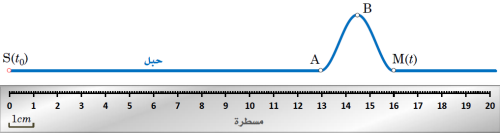
\includegraphics[width=0.6\textwidth ]{./img/Exercice01.png}
  %\end{center}



\begin{Box2}{\textbf{Exercice 1 :Utilisation des ondes ultra sonores dans le contrôle du béton armé  }
	}
	   \textbf{1. Détermination de la vitesse de propagation des ondes ultrasonores dans l’air :}

	   Sur une même droite on place un émetteur (E) et un récepteur (R) des ondes ultrasonores
distants de d=0,5m.

L’émetteur (E) envoie un signal, il est reçu par le récepteur (R) après $\tau$=$1,47ms$

\textbf{1.1- }Dites si les ondes ultrasonores sont longitudinales ou transversales

\textbf{1.2- }Donner la signification physique de la grandeur $\tau$.

\textbf{1.3- }Calculer la valeur Vair de la vitesse de propagation des ondes ultrasonores dans l’air.

\textbf{1.4- }On considère un point B situe à une distance dB de l’émetteur (E). sélectionner la réponse
juste parmi ces propositions :

\textbf{(a):}$y_B(t)=y_E(t-\tau_B)$ --- \textbf{(b):}$y_B(t)=y_E(t+\tau_B)$ --- \textbf{(c):}$y_B(t)=y_E(t-2\tau_B)$ --- \textbf{(d):}$y_B(t)=y_E(t-\tau_B/2)$


\textbf{2- Contrôle de la qualité du béton armé à l’aide des ondes ultra sonores:}

L’oscillogramme de la figure ci-dessous représente le signal émis par un émetteur (E) d’un
appareil numérique de contrôle du béton armé fixe sur la paroi d’un mur et le signal reçu par
un récepteur (R) du même appareil placé sur l’autre paroi du mur d’une épaisseur e=60cm.
La qualité du béton arme dépend de la vitesse de propagation des ondes ultrasonores dans ce
béton comme l’indique le tableau ci-dessous.
\begin{wrapfigure}[2]{r}{0.48\textwidth}
  \begin{center}
	  \vspace{-1cm}
	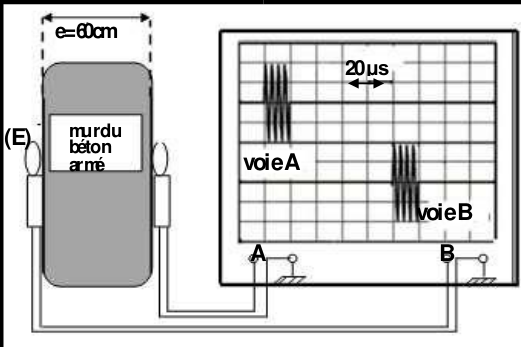
\includegraphics[width=0.48\textwidth]{./img/ex1.png}
  \end{center}
\end{wrapfigure}

\begin{tabular}{ |c|c| } 
 \hline
 \makecell{ \textbf{Qualité du}\\\textbf{béton armé}} & \makecell{\textbf{Vitesse de propagation}\\\textbf{des ondes ultrasonores}\\\textbf{dans le béton arme (m/s)} }  \\\hline

 excellente & Supérieure à 4000  \\\hline
 bonne & De 3200 à 4000  \\\hline 
 acceptable & De 2500 à 3200  \\\hline 
 mauvaise & De 1700 à 2500 \\\hline 
 Très mauvaise & Inférieure à 1700  \\\hline 
 \hline
\end{tabular}

Trouver la valeur de v la vitesse de propagation

des ondes ultra sonore dans le béton arme et 

déduire sa qualité.
%\vspace{1cm}
\end{Box2}
%%_________________________Exercice !2 :"_________________________Exercice
\begin{tcolorbox}\textbf{Exercice 2 : propagation d’ondes ultrasonores et des ondes lumineuses }
\end{tcolorbox}
%\begin{wrapfigure}{r}{0.22\textwidth}
  %\begin{center}
	  %\vspace{-0.6cm}
	%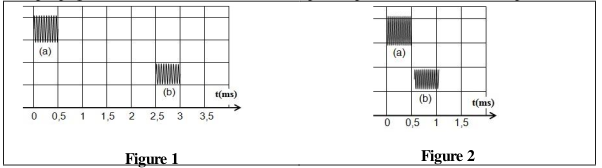
\includegraphics[width=0.22\textwidth]{./img/Ex2.png}
  %\end{center}
%\end{wrapfigure}

	\emph{Les ondes mécaniques et les ondes lumineuses sont caractérisées par des propriétés bien
déterminées. Les phénomènes liés à leur propagation permettent de fournir des informations sur
les milieux de propagation et la nature de la lumière, et de déterminer certains paramètres
caractéristiques.}

\textbf{1- Propriétés des ondes ultrasonores et des ondes lumineuses:}

Recopier sur votre copie, le numéro de la question, et écrire la lettre correspondante à la
seule proposition vraie parmi :


\begin{tabular}{ |l|l| } 
 \hline
a & les ondes ultrasonores sont des ondes longitudinales.   \\\hline
 b & Le domaine de fréquences de la lumière visible est limité entre $400 nm$ et $1000 nm$.  \\\hline
 c & \makecell{les ondes ultrasonores et les ondes lumineuses ont même célérité de propagation\\dans
 le même milieu.}  \\\hline 
 d & La fréquence des ondes lumineuses varie d’un milieu à un autre.  \\\hline 
 \hline
\end{tabular}

\textbf{2- Propagation des ondes ultrasonores:}

On place en une même position, un émetteur E et un récepteur R des ondes ultrasonores, à la
distance d=42,5 cm d’un obstacle. Les ondes ultrasonores qui se propagent à partir de E, se
réfléchissent sur
l’obstacle puis sont reçues par R.
Un système d’acquisition informatique permet de visualiser l’onde émise (a)et l’onde reçue(b).
La figure (1) donne l’oscillogramme obtenu.

\textbf{2.1- }Déterminer la valeur du retard temporel $\tau$ entre les ondes (a) et (b).

\textbf{2.2- }Vérifier que la valeur de la célérité de propagation dans l’air est $V_{air}$=$340 m/s$.

\textbf{2.3- }On répète l’expérience en utilisant le même dispositif, et l’eau comme milieu de
propagation. On obtient avec le même système d’acquisition informatique
l’oscillogramme représenté sur la figure (2). Dans quel milieu (air/eau), la
propagation des ondes ultrasonores est plus rapide ? Justifier votre réponse.

  \begin{center}
	  \vspace{-0.4cm}
	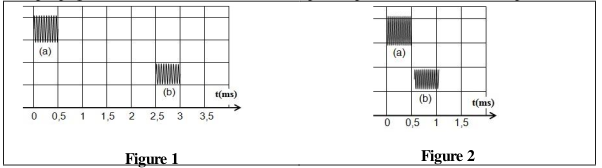
\includegraphics[width=0.8\textwidth]{./img/Ex2.png}
  \end{center}

%%_________________________Exercice ! 3:"_________________________Exercice

	  \vspace{-0.5cm}
  \begin{Box2}{\textbf{Exercice 3 :  L’échographie et les ondes ultrasonores  }}
\emph{L’échographie utilisant les ondes ultrasonores est une méthode de détermination des épaisseurs
des nappes souterraines.
Cet exercice vise à déterminer, la célérité de propagation des ondes ultrasonores dans l’air,
ainsi que l’épaisseur d’une nappe souterraine de pétrole}

\underline{\textbf{1- Détermination de la célérité des ondes ultrasonores dans l’air :}}

On place sur un banc rectiligne un émetteur E d’ondes ultrasonores, et deux récepteurs R1 et R2
distants de d=0,5m (Figure 1).

On visualise sur l’écran d’un oscilloscope, aux entrées Y1 et Y2, les signaux reçus par les deux
récepteurs, On obtient l’oscillogramme représenté sur la figure 2.

A représente le début du signal reçu par R1, et B le début de celui reçu par R2.

  \begin{center}
	  \vspace{-0.5cm}
	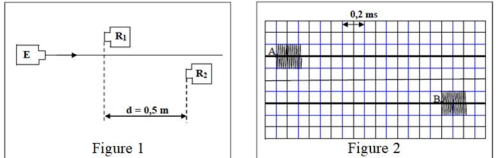
\includegraphics[width=0.65\textwidth]{./img/ex3_1.png}
  \end{center}

  \textbf{1.1- }Déterminer à partir de l’oscillogramme de la figure 2, le retard horaire $\tau$ entre les deux
signaux reçus par les deux récepteurs R1 et R2.

\textbf{1.2- }Calculer $V_{air}$ la vitesse de propagation des ondes ultrasonores dans l’air.

\textbf{1-3- }Ecrire l’expression de l’élongation $y_B(t)$ du point B à l’instant t, en fonction de l’élongation du point A.

\underline{\textbf{2 - Détermination de l ’épaisseur d’une nappe souterraine de pétrole :}}

\begin{wrapfigure}[8]{r}{0.22\textwidth}
  \begin{center}
	  \vspace{-1.5cm}
	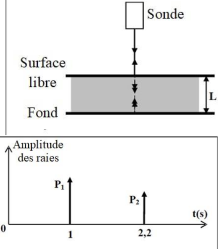
\includegraphics[width=0.22\textwidth]{./img/ex3_2.png}
  \end{center}
\end{wrapfigure}


Pour déterminer l’épaisseur L d’une nappe souterraine de
pétrole, un ingénieur utilise la sonde d’un appareil
d’échographie.

La sonde envoie, perpendiculairement à la surface libre de la
couche de pétrole, à l’instant $t_0 = 0$, un signal ultrasonore de
très courte durée.

Une partie du signal se réfléchie sur cette surface, tandis que
l’autre partie continue la propagation dans la couche de
pétrole pour se réfléchir une deuxième fois sur son fond, et
revenir vers la sonde, pour être
transformée à nouveau
en un signal de très courte durée aussi (Figure 3).

A l’instant $t_1$, la sonde révèle la raie $P_1$ correspondante à
l’onde réfléchie sur la surface libre de la couche de pétrole,
et à l’instant $t_2$ elle révèle la raie $P_2$ correspondante à l’onde
réfléchie sur le fond de la couche du pétrole (Figure 4).


\textbf{Déterminer l’épaisseur L de la couche de pétrole, sachant que la célérité de propagation des ondes
ultrasonores dans le pétrole brut est : $V = 1,3 km.s^{-1}$.}
\end{Box2}



\begin{Box2}{\textbf{Exercice 4 : la célérité de propagation d’une onde le long d’une corde}}

\begin{wrapfigure}[11]{r}{0.32\textwidth}
  \begin{center}
	  \vspace{-0.5cm}
	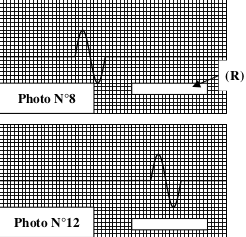
\includegraphics[width=0.32\textwidth]{./img/ex4.png}
  \end{center}
\end{wrapfigure}



\emph{Pour déterminer la célérité de propagation d’une onde le long d’une corde, le professeur de
physique demande à l’un des élèves de produire un ébranlement à l’une des extrémités d’une corde
horizontale, et en même temps, il demande à une élève de
filmer la séquence à l’aide d’une caméra numérique réglée sur
la prise de 25 images par seconde.}

Une règle blanche (R) de longueur 1 m, a été placée au
(R)
voisinage de la corde comme échelle de mesure.

Après traitement informatique avec un logiciel convenable, le
professeur choisit parmi les photos obtenues, les photos N°8 et
N°12 (Figure ci-dessus), pour les étudier et les exploiter.

\textbf{1- }Déterminer La durée $\Delta{t}$ séparant la prise des deux photos N°8 et N°12 de l’onde.

\textbf{2- }Déterminer La distance d parcourue par l’onde pendant la durée 
$\Delta{t}$. 

\textbf{3- }La célérité de propagation de l’onde le long de la corde.
\end{Box2}

\begin{Box2}{\textbf{Exercice 5 : la célérité d’une onde ultrasonore dans le pétrole
liquide }}

\emph{Pour déterminer la valeur approximative de la célérité d’une onde ultrasonore dans le pétrole
liquide on réalise l’expérience suivante :}

Dans une cuve contenant du pétrole, on fixe à l’une de ses extrémités deux émetteurs $E_1$ et $E_2$ qui
sont reliés à un générateur GBF. A l’instant $t_0$=0s, les deux émetteurs émettent chacun une onde
ultrasonore, une se propage dans l’air et l’autre dans le pétrole. A l’autre extrémité de la cuve, on
place deux récepteurs $R_1$ et $R_2$, l’un dans l’air et l’autre dans le pétrole. Les récepteurs sont à une
distance L des émetteurs. (Voir figure 1)

On visualise sur l’écran d’un oscilloscope les deux signaux reçus par $R_1$ et $R_2$. (Voir figure 2)

\underline{Données :} 
\begin{itemize}
	\item Les deux ondes parcourent la même distance L = 1,84 m .
	\item La célérité des ultrasons dans l’air : $V_{air} = 340 m.s^{-1}$.
	\item La sensibilité horizontale de l’oscilloscope : 2ms/div.
\end{itemize}

\textbf{1- }Les ondes ultrasonores, sont-elles longitudinales ou transversales ? justifier.

\textbf{2- }En exploitant la figure 2, déterminer la valeur du retard temporel entre les deux ondes reçues.

\textbf{3- }Montrer que l’expression de s’écrit sous la forme : $\tau$=$L.(\frac{1}{V_{air}} - \frac{1}{V_P})$

\textbf{4- }Trouver la valeur approchée de la célérité.
 \begin{center}
	  %\vspace{-1cm}
	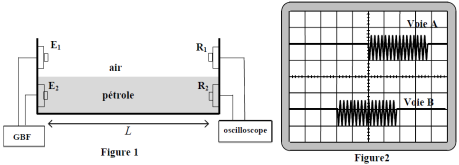
\includegraphics[width=0.62\textwidth]{./img/ex5.png}
  \end{center}
\end{Box2}


\begin{Box2}{\textbf{Exercice 6 : la célérité d’une onde ultrasonore dans le pétrole
liquide }}


\begin{wrapfigure}[15]{r}{0.32\textwidth}
  \begin{center}
	  \vspace{-0.56cm}
	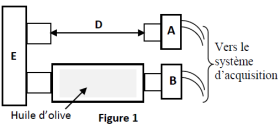
\includegraphics[width=0.32\textwidth]{./img/ex6_1.png}
	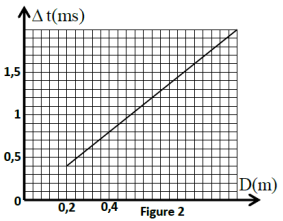
\includegraphics[width=0.32\textwidth]{./img/ex6_2.png}
  \end{center}
\end{wrapfigure}



L’émetteur E d’ultrasons génère simultanément deux
salves d’ondes. Les récepteurs A et B sont reliés à une
interface d’acquisition qui déclenche l’enregistrement
des signaux dès que le récepteur B détecte en premier les
ultrasons. L’huile testée est disposée dans un tube en
verre entre l’émetteur E et le récepteur B, tandis que l’air
sépare l’émetteur E du récepteur A (figure 1).
Pour chaque valeur D de la longueur du tube on mesure, par l’intermédiaire du système
informatique, la durée $\Delta{t}$ écoulée entre les deux signaux
reçus en A et B.

À partir de ces mesures on obtient la courbe de la figure
2 représentant les variations de $\Delta{t}$ en
fonction de D : $\Delta{t}$=f(D).

\textbf{1- }Les ondes ultrasonores sont-elles des ondes
longitudinales ou transversales ? Justifier.

\textbf{2- }Les ultrasons utilisés dans l’expérience
précédente ont une fréquence de $40 kHz$. Leur
célérité dans l’air est $V_a$=$340m/s$.

Calculer la distance parcourue par ces ultrasons
dans l’air pendant une période.

\textbf{3- }Exprimer $\Delta{t}$ en fonction de D, $V_h$ et $V_a$

\textbf{4- }L’huile testée est-t-elle pure ? Justifier.

\end{Box2}

\begin{tcolorbox} \textbf{Exercice 7 :Vitesse de propagation des ondes ultrasonores }
\end{tcolorbox}
	\emph{Les ondes ultrasonores sont des ondes mécaniques qui peuvent se propager dans les liquides
avec une vitesse qui dépend de la nature du liquide et de la vitesse de son écoulement.
L’objectif de cet exercice est de déterminer la vitesse d’écoulement de l’eau dans une conduite.}

\textbf{1- \underline{Propagation d’une onde ultrasonore:}}
une onde ultrasonore de fréquence $N=50Hz$ se propagent dans une eau calme avec une vitesse
$v_0$=$1500 m.s^{-1}$.

\textbf{1.1- }Calculer la longueur d’onde $\lambda$ de cette onde ultrasonore se propageant dans une eau calme.

\textbf{1.2- }La valeur de $\lambda$ varie-t-elle si cette onde se propage dans l’air ? Justifier la réponse.

\textbf{2- \underline{Mesure de la vitesse d’écoulement de l’eau dans une conduite :}}

Une onde ultrasonore se propage à la vitesse v dans une eau qui coule à la vitesse ve dans une
conduite tel que $\vec{v} = \vec{v_0} + \vec{v_e}$ avec $\vec{v_e}$ vecteur vitesse de propagation de cette onde dans une eau calme.
\\Pour déterminer la vitesse $v_e$ d’écoulement de l’eau dans une conduite horizontale, on y place un
émetteur E et un récepteur R d’ondes ultrasonores.
\\L’émetteur E et le récepteur R sont situés sur la même droite horizontale et parallèle à la direction
du mouvement de l’eau et sont séparés d’une distance $d=1,0m$.
\\L’émetteur E émet une onde ultrasonore de faible durée qui est reçue par le récepteur R.
\\Un dispositif adéquat permet d’enregistrer le signal $u(t)$ reçu par le récepteur R. On enregistre le
signal $u(t)$ dans les deux cas suivants :

\textbf{ \underline{- 1er cas :}} L’émetteur E est à la position A, et le récepteur R est à la position B (figure1).

\textbf{\underline{- 2eme cas :}} L’émetteur E est à la position B, et le récepteur R est à la position A (figure2).
On considère, pour chaque cas, l’instant de l’émission de l’onde ultrasonore par l’émetteur E comme
origine des dates.

  \begin{center}
	  \vspace{-0.56cm}
	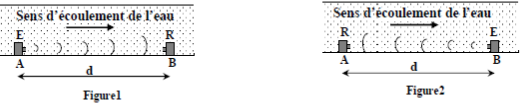
\includegraphics[width=0.7\textwidth]{./img/ex7_1.png}
  \end{center}


\begin{wrapfigure}[8]{r}{0.42\textwidth}
  \begin{center}
	  \vspace{-0.6cm}
	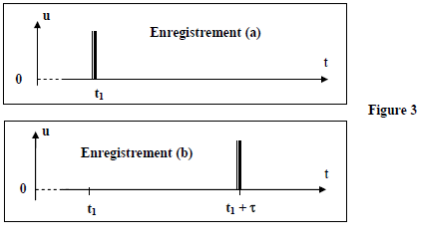
\includegraphics[width=0.42\textwidth]{./img/ex7_2.png}
  \end{center}
\end{wrapfigure}




  La figure 3 représente les deux enregistrements obtenus (a) et (b).

  \textbf{2.1- }Indiquer l’enregistrement correspondant au 2ème cas. Justifier la réponse.

  \textbf{2.2- }$\tau$ représente la différence des deux durées de propagation de l’onde ultrasonore de l’émetteur E au récepteur R dans les deux cas.

  \textbf{2.2.a- }Déterminer l’expression de $\tau$ en fonction de $v_e$, $v_0$ et d.

  \textbf{2.2.b- }En négligeant la vitesse $v_e$ devant $v_0$, déterminer la vitesse $v_e$ d’écoulement de l’eau dans la conduite sachant que $\tau= 2,0 \mu s$.



%%_________________________Exercice 4 : _________________________Exercice
\begin{Box2}{Exercice 8 :La vitesse de propagation de l’onde ultrasonore dans le plexiglas }

	\begin{wrapfigure}[12]{r}{0.42\textwidth}
  \begin{center}
	  \vspace{-0.6cm}
	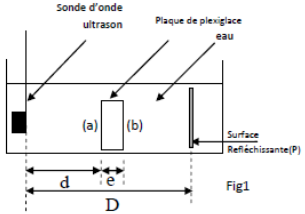
\includegraphics[width=0.42\textwidth]{./img/ex8_1.png}
  \end{center}
\end{wrapfigure}



	\emph{On place dans un récipient contenant de l’eau,
une plaque de plexiglas d’épaisseur e, on plonge
dans l’eau une sonde constituée d’un émetteur et
d’un récepteur d’onde ultrasonore (figure1) On
visualise à l’aide d’un dispositif approprié chacun
des signaux émis et reçu par la sonde. La durée du
signal ultrasonore est très petite, on le représente
par une raie verticale.
}

\textbf{1- }En l’absence de la plaque du plexiglas, on
obtient l’oscillogramme représenté dans la
figure 2.

Etablir que l’instant $t_R$ auquel a été capté le
Signal réfléchi par la surface réfléchissante (P) s’écrit sous la forme $t_R = \frac{2D}{v}$ 
où v est la vitesse de propagation de l’onde ultrasonore dans l’eau.

\textbf{2- }En présence de la plaque de plexiglas , on obtient l’oscillogramme de la figure 3.

On représente par $t_A$ et $t_B$ les instants auxquels sont captés les signaux réfléchis successivement
par la première surfaces (a) et la deuxième surface (b) de la plaque de plexiglas.

On représente par $t’_R$ l’instant auquel a été captée l’onde réfléchie sur la surface réfléchissante
(P).

On représente la vitesse de propagation de l’onde ultrasonore dans le plexiglas par v’

\textbf{2.1- }Dans quel milieu (eau ou plexiglas), La vitesse de propagation de l’onde est la plus Grande
? justifier la réponse.

\textbf{2.2- }Exprimer $t’_R$ en fonction de D, e, v et v’.

\textbf{2.3- }Trouver l’expression de l’épaisseur e en fonction de v, $t_R$, $t’_R$, $t_A$ et $t_B$.

Calculer la valeur de e sachant que la vitesse de propagation des ondes ultrasonores dans
l’eau est $v$=$1,42.10^3 m.s^{-1}$.

\begin{center}
	  %\vspace{-0.6cm}
	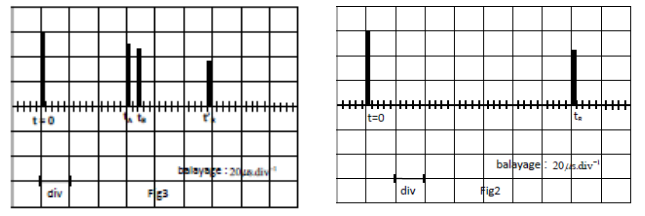
\includegraphics[width=1\textwidth]{./img/ex8_2.png}
  \end{center}

\end{Box2}
%\vspace{2cm}
%\begin{center}
   %\Large{ \em{Exercices Supplémentaires}}
%\end{center}


%\vspace{-0.7cm}
%%_________________________Exercice 5 : _________________________Exercice
%\begin{Box2}{Exercice 5 :Les ondes sonores }
%4
%\end{Box2}
%%_________________________Exercice 6 : _________________________Exercice
%\begin{Box2}{Exercice 6 : échographie}
%6
%\end{Box2}

\end{document}
